\documentclass[1p]{elsarticle_modified}
%\bibliographystyle{elsarticle-num}

%\usepackage[colorlinks]{hyperref}
%\usepackage{abbrmath_seonhwa} %\Abb, \Ascr, \Acal ,\Abf, \Afrak
\usepackage{amsfonts}
\usepackage{amssymb}
\usepackage{amsmath}
\usepackage{amsthm}
\usepackage{scalefnt}
\usepackage{amsbsy}
\usepackage{kotex}
\usepackage{caption}
\usepackage{subfig}
\usepackage{color}
\usepackage{graphicx}
\usepackage{xcolor} %% white, black, red, green, blue, cyan, magenta, yellow
\usepackage{float}
\usepackage{setspace}
\usepackage{hyperref}

\usepackage{tikz}
\usetikzlibrary{arrows}

\usepackage{multirow}
\usepackage{array} % fixed length table
\usepackage{hhline}

%%%%%%%%%%%%%%%%%%%%%
\makeatletter
\renewcommand*\env@matrix[1][\arraystretch]{%
	\edef\arraystretch{#1}%
	\hskip -\arraycolsep
	\let\@ifnextchar\new@ifnextchar
	\array{*\c@MaxMatrixCols c}}
\makeatother %https://tex.stackexchange.com/questions/14071/how-can-i-increase-the-line-spacing-in-a-matrix
%%%%%%%%%%%%%%%

\usepackage[normalem]{ulem}

\newcommand{\msout}[1]{\ifmmode\text{\sout{\ensuremath{#1}}}\else\sout{#1}\fi}
%SOURCE: \msout is \stkout macro in https://tex.stackexchange.com/questions/20609/strikeout-in-math-mode

\newcommand{\cancel}[1]{
	\ifmmode
	{\color{red}\msout{#1}}
	\else
	{\color{red}\sout{#1}}
	\fi
}

\newcommand{\add}[1]{
	{\color{blue}\uwave{#1}}
}

\newcommand{\replace}[2]{
	\ifmmode
	{\color{red}\msout{#1}}{\color{blue}\uwave{#2}}
	\else
	{\color{red}\sout{#1}}{\color{blue}\uwave{#2}}
	\fi
}

\newcommand{\Sol}{\mathcal{S}} %segment
\newcommand{\D}{D} %diagram
\newcommand{\A}{\mathcal{A}} %arc


%%%%%%%%%%%%%%%%%%%%%%%%%%%%%5 test

\def\sl{\operatorname{\textup{SL}}(2,\Cbb)}
\def\psl{\operatorname{\textup{PSL}}(2,\Cbb)}
\def\quan{\mkern 1mu \triangleright \mkern 1mu}

\theoremstyle{definition}
\newtheorem{thm}{Theorem}[section]
\newtheorem{prop}[thm]{Proposition}
\newtheorem{lem}[thm]{Lemma}
\newtheorem{ques}[thm]{Question}
\newtheorem{cor}[thm]{Corollary}
\newtheorem{defn}[thm]{Definition}
\newtheorem{exam}[thm]{Example}
\newtheorem{rmk}[thm]{Remark}
\newtheorem{alg}[thm]{Algorithm}

\newcommand{\I}{\sqrt{-1}}
\begin{document}

%\begin{frontmatter}
%
%\title{Boundary parabolic representations of knots up to 8 crossings}
%
%%% Group authors per affiliation:
%\author{Yunhi Cho} 
%\address{Department of Mathematics, University of Seoul, Seoul, Korea}
%\ead{yhcho@uos.ac.kr}
%
%
%\author{Seonhwa Kim} %\fnref{s_kim}}
%\address{Center for Geometry and Physics, Institute for Basic Science, Pohang, 37673, Korea}
%\ead{ryeona17@ibs.re.kr}
%
%\author{Hyuk Kim}
%\address{Department of Mathematical Sciences, Seoul National University, Seoul 08826, Korea}
%\ead{hyukkim@snu.ac.kr}
%
%\author{Seokbeom Yoon}
%\address{Department of Mathematical Sciences, Seoul National University, Seoul, 08826,  Korea}
%\ead{sbyoon15@snu.ac.kr}
%
%\begin{abstract}
%We find all boundary parabolic representation of knots up to 8 crossings.
%
%\end{abstract}
%\begin{keyword}
%    \MSC[2010] 57M25 
%\end{keyword}
%
%\end{frontmatter}

%\linenumbers
%\tableofcontents
%
\newcommand\colored[1]{\textcolor{white}{\rule[-0.35ex]{0.8em}{1.4ex}}\kern-0.8em\color{red} #1}%
%\newcommand\colored[1]{\textcolor{white}{ #1}\kern-2.17ex	\textcolor{white}{ #1}\kern-1.81ex	\textcolor{white}{ #1}\kern-2.15ex\color{red}#1	}

{\Large $\underline{12n_{0181}~(K12n_{0181})}$}

\setlength{\tabcolsep}{10pt}
\renewcommand{\arraystretch}{1.6}
\vspace{1cm}\begin{tabular}{m{100pt}>{\centering\arraybackslash}m{274pt}}
\multirow{5}{120pt}{
	\centering
	\includegraphics[width=112pt]{../../../GIT/diagram.site/Diagrams/png/2270_12n_0181.png}\\
\ \ \ A knot diagram\footnotemark}&
\allowdisplaybreaks
\textbf{Linearized knot diagam} \\
\cline{2-2}
 &
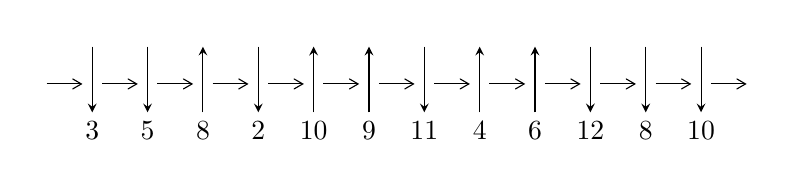
\begin{tikzpicture}[x=20pt, y=17pt]
	% nodes
	\node (C0) at (0, 0) {};
	\node (C1) at (1, 0) {};
	\node (C1U) at (1, +1) {};
	\node (C1D) at (1, -1) {3};

	\node (C2) at (2, 0) {};
	\node (C2U) at (2, +1) {};
	\node (C2D) at (2, -1) {5};

	\node (C3) at (3, 0) {};
	\node (C3U) at (3, +1) {};
	\node (C3D) at (3, -1) {8};

	\node (C4) at (4, 0) {};
	\node (C4U) at (4, +1) {};
	\node (C4D) at (4, -1) {2};

	\node (C5) at (5, 0) {};
	\node (C5U) at (5, +1) {};
	\node (C5D) at (5, -1) {10};

	\node (C6) at (6, 0) {};
	\node (C6U) at (6, +1) {};
	\node (C6D) at (6, -1) {9};

	\node (C7) at (7, 0) {};
	\node (C7U) at (7, +1) {};
	\node (C7D) at (7, -1) {11};

	\node (C8) at (8, 0) {};
	\node (C8U) at (8, +1) {};
	\node (C8D) at (8, -1) {4};

	\node (C9) at (9, 0) {};
	\node (C9U) at (9, +1) {};
	\node (C9D) at (9, -1) {6};

	\node (C10) at (10, 0) {};
	\node (C10U) at (10, +1) {};
	\node (C10D) at (10, -1) {12};

	\node (C11) at (11, 0) {};
	\node (C11U) at (11, +1) {};
	\node (C11D) at (11, -1) {8};

	\node (C12) at (12, 0) {};
	\node (C12U) at (12, +1) {};
	\node (C12D) at (12, -1) {10};
	\node (C13) at (13, 0) {};

	% arrows
	\draw[->,>={angle 60}]
	(C0) edge (C1) (C1) edge (C2) (C2) edge (C3) (C3) edge (C4) (C4) edge (C5) (C5) edge (C6) (C6) edge (C7) (C7) edge (C8) (C8) edge (C9) (C9) edge (C10) (C10) edge (C11) (C11) edge (C12) (C12) edge (C13) ;	\draw[->,>=stealth]
	(C1U) edge (C1D) (C2U) edge (C2D) (C3D) edge (C3U) (C4U) edge (C4D) (C5D) edge (C5U) (C6D) edge (C6U) (C7U) edge (C7D) (C8D) edge (C8U) (C9D) edge (C9U) (C10U) edge (C10D) (C11U) edge (C11D) (C12U) edge (C12D) ;
	\end{tikzpicture} \\
\hhline{~~} \\& 
\textbf{Solving Sequence} \\ \cline{2-2} 
 &
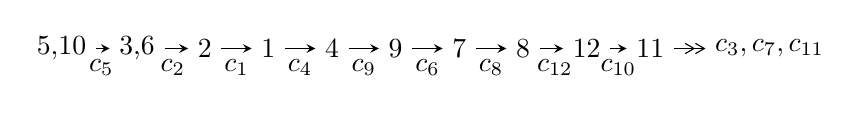
\begin{tikzpicture}[x=23pt, y=7pt]
	% node
	\node (A0) at (-1/8, 0) {5,10};
	\node (A1) at (17/16, 0) {3,6};
	\node (A2) at (17/8, 0) {2};
	\node (A3) at (25/8, 0) {1};
	\node (A4) at (33/8, 0) {4};
	\node (A5) at (41/8, 0) {9};
	\node (A6) at (49/8, 0) {7};
	\node (A7) at (57/8, 0) {8};
	\node (A8) at (65/8, 0) {12};
	\node (A9) at (73/8, 0) {11};
	\node (C1) at (1/2, -1) {$c_{5}$};
	\node (C2) at (13/8, -1) {$c_{2}$};
	\node (C3) at (21/8, -1) {$c_{1}$};
	\node (C4) at (29/8, -1) {$c_{4}$};
	\node (C5) at (37/8, -1) {$c_{9}$};
	\node (C6) at (45/8, -1) {$c_{6}$};
	\node (C7) at (53/8, -1) {$c_{8}$};
	\node (C8) at (61/8, -1) {$c_{12}$};
	\node (C9) at (69/8, -1) {$c_{10}$};
	\node (A10) at (11, 0) {$c_{3},c_{7},c_{11}$};

	% edge
	\draw[->,>=stealth]	
	(A0) edge (A1) (A1) edge (A2) (A2) edge (A3) (A3) edge (A4) (A4) edge (A5) (A5) edge (A6) (A6) edge (A7) (A7) edge (A8) (A8) edge (A9) ;
	\draw[->>,>={angle 60}]	
	(A9) edge (A10);
\end{tikzpicture} \\ 

\end{tabular} \\

\footnotetext{
The image of knot diagram is generated by the software ``\textbf{Draw programme}" developed by Andrew Bartholomew(\url{http://www.layer8.co.uk/maths/draw/index.htm\#Running-draw}), where we modified some parts for our purpose(\url{https://github.com/CATsTAILs/LinksPainter}).
}\phantom \\ \newline 
\centering \textbf{Ideals for irreducible components\footnotemark of $X_{\text{par}}$} 
 
\begin{align*}
I^u_{1}&=\langle 
-2.89597\times10^{103} u^{52}+7.97404\times10^{103} u^{51}+\cdots+3.42001\times10^{105} b-2.68164\times10^{105},\\
\phantom{I^u_{1}}&\phantom{= \langle  }-2.24253\times10^{103} u^{52}+6.90313\times10^{103} u^{51}+\cdots+1.36801\times10^{105} a-2.45570\times10^{105},\\
\phantom{I^u_{1}}&\phantom{= \langle  }u^{53}-3 u^{52}+\cdots-49 u+49\rangle \\
I^u_{2}&=\langle 
-1878 a^5 u+2600 a^4 u+\cdots+23830 a-8647,\\
\phantom{I^u_{2}}&\phantom{= \langle  }a^6-3 a^5 u-4 a^5+7 a^4 u- a^4- a^3 u-3 a^3+9 a^2 u+5 a^2-6 a u+2 a+u,\;u^2+1\rangle \\
\\
\end{align*}
\raggedright * 2 irreducible components of $\dim_{\mathbb{C}}=0$, with total 65 representations.\\
\footnotetext{All coefficients of polynomials are rational numbers. But the coefficients are sometimes approximated in decimal forms when there is not enough margin.}
\newpage
\renewcommand{\arraystretch}{1}
\centering \section*{I. $I^u_{1}= \langle -2.90\times10^{103} u^{52}+7.97\times10^{103} u^{51}+\cdots+3.42\times10^{105} b-2.68\times10^{105},\;-2.24\times10^{103} u^{52}+6.90\times10^{103} u^{51}+\cdots+1.37\times10^{105} a-2.46\times10^{105},\;u^{53}-3 u^{52}+\cdots-49 u+49 \rangle$}
\flushleft \textbf{(i) Arc colorings}\\
\begin{tabular}{m{7pt} m{180pt} m{7pt} m{180pt} }
\flushright $a_{5}=$&$\begin{pmatrix}1\\0\end{pmatrix}$ \\
\flushright $a_{10}=$&$\begin{pmatrix}0\\u\end{pmatrix}$ \\
\flushright $a_{3}=$&$\begin{pmatrix}0.0163927 u^{52}-0.0504613 u^{51}+\cdots+4.67289 u+1.79509\\0.00846773 u^{52}-0.0233158 u^{51}+\cdots+3.33538 u+0.784101\end{pmatrix}$ \\
\flushright $a_{6}=$&$\begin{pmatrix}1\\- u^2\end{pmatrix}$ \\
\flushright $a_{2}=$&$\begin{pmatrix}0.0248604 u^{52}-0.0737771 u^{51}+\cdots+8.00826 u+2.57919\\0.00846773 u^{52}-0.0233158 u^{51}+\cdots+3.33538 u+0.784101\end{pmatrix}$ \\
\flushright $a_{1}=$&$\begin{pmatrix}-0.00350318 u^{52}+0.0151353 u^{51}+\cdots-5.53251 u+4.45074\\0.00290112 u^{52}-0.00548627 u^{51}+\cdots-1.43147 u+1.55122\end{pmatrix}$ \\
\flushright $a_{4}=$&$\begin{pmatrix}-0.0134120 u^{52}+0.0381751 u^{51}+\cdots-12.1908 u+0.357746\\-0.00827306 u^{52}+0.0265007 u^{51}+\cdots-4.74375 u+0.368964\end{pmatrix}$ \\
\flushright $a_{9}=$&$\begin{pmatrix}- u\\u^3+u\end{pmatrix}$ \\
\flushright $a_{7}=$&$\begin{pmatrix}u^2+1\\- u^4-2 u^2\end{pmatrix}$ \\
\flushright $a_{8}=$&$\begin{pmatrix}0.0238148 u^{52}-0.0757412 u^{51}+\cdots+15.3375 u-0.149255\\0.0114699 u^{52}-0.0338179 u^{51}+\cdots+7.34993 u-0.181045\end{pmatrix}$ \\
\flushright $a_{12}=$&$\begin{pmatrix}-0.00350318 u^{52}+0.0151353 u^{51}+\cdots-5.53251 u+4.45074\\0.00182181 u^{52}-0.00371679 u^{51}+\cdots-1.82979 u+1.77789\end{pmatrix}$ \\
\flushright $a_{11}=$&$\begin{pmatrix}-0.0209597 u^{52}+0.0608672 u^{51}+\cdots-11.6241 u-1.93839\\-0.00957219 u^{52}+0.0293318 u^{51}+\cdots-5.11792 u-0.541740\end{pmatrix}$\\&\end{tabular}
\flushleft \textbf{(ii) Obstruction class $= -1$}\\~\\
\flushleft \textbf{(iii) Cusp Shapes $= 0.0668454 u^{52}-0.159654 u^{51}+\cdots+29.7015 u+4.20227$}\\~\\
\newpage\renewcommand{\arraystretch}{1}
\flushleft \textbf{(iv) u-Polynomials at the component}\newline \\
\begin{tabular}{m{50pt}|m{274pt}}
Crossings & \hspace{64pt}u-Polynomials at each crossing \\
\hline $$\begin{aligned}c_{1}\end{aligned}$$&$\begin{aligned}
&u^{53}+33 u^{52}+\cdots-47 u+1
\end{aligned}$\\
\hline $$\begin{aligned}c_{2},c_{4}\end{aligned}$$&$\begin{aligned}
&u^{53}-5 u^{52}+\cdots- u+1
\end{aligned}$\\
\hline $$\begin{aligned}c_{3},c_{8}\end{aligned}$$&$\begin{aligned}
&u^{53}+u^{52}+\cdots-3 u+1
\end{aligned}$\\
\hline $$\begin{aligned}c_{5},c_{6},c_{9}\end{aligned}$$&$\begin{aligned}
&u^{53}+3 u^{52}+\cdots-49 u-49
\end{aligned}$\\
\hline $$\begin{aligned}c_{7},c_{11}\end{aligned}$$&$\begin{aligned}
&u^{53}+3 u^{52}+\cdots-55 u-17
\end{aligned}$\\
\hline $$\begin{aligned}c_{10},c_{12}\end{aligned}$$&$\begin{aligned}
&u^{53}+31 u^{52}+\cdots-613 u+289
\end{aligned}$\\
\hline
\end{tabular}\\~\\
\newpage\renewcommand{\arraystretch}{1}
\flushleft \textbf{(v) Riley Polynomials at the component}\newline \\
\begin{tabular}{m{50pt}|m{274pt}}
Crossings & \hspace{64pt}Riley Polynomials at each crossing \\
\hline $$\begin{aligned}c_{1}\end{aligned}$$&$\begin{aligned}
&y^{53}-21 y^{52}+\cdots+1053 y-1
\end{aligned}$\\
\hline $$\begin{aligned}c_{2},c_{4}\end{aligned}$$&$\begin{aligned}
&y^{53}-33 y^{52}+\cdots-47 y-1
\end{aligned}$\\
\hline $$\begin{aligned}c_{3},c_{8}\end{aligned}$$&$\begin{aligned}
&y^{53}-9 y^{52}+\cdots+25 y-1
\end{aligned}$\\
\hline $$\begin{aligned}c_{5},c_{6},c_{9}\end{aligned}$$&$\begin{aligned}
&y^{53}+63 y^{52}+\cdots-67963 y-2401
\end{aligned}$\\
\hline $$\begin{aligned}c_{7},c_{11}\end{aligned}$$&$\begin{aligned}
&y^{53}-31 y^{52}+\cdots-613 y-289
\end{aligned}$\\
\hline $$\begin{aligned}c_{10},c_{12}\end{aligned}$$&$\begin{aligned}
&y^{53}-11 y^{52}+\cdots+7632559 y-83521
\end{aligned}$\\
\hline
\end{tabular}\\~\\
\newpage\flushleft \textbf{(vi) Complex Volumes and Cusp Shapes}
$$\begin{array}{c|c|c}  
\text{Solutions to }I^u_{1}& \I (\text{vol} + \sqrt{-1}CS) & \text{Cusp shape}\\
 \hline 
\begin{aligned}
u &= -0.595173 + 0.790194 I \\
a &= \phantom{-}0.44043 + 1.93505 I \\
b &= -1.210360 - 0.280896 I\end{aligned}
 & -4.60939 - 3.81170 I & -6.73528 + 3.84171 I \\ \hline\begin{aligned}
u &= -0.595173 - 0.790194 I \\
a &= \phantom{-}0.44043 - 1.93505 I \\
b &= -1.210360 + 0.280896 I\end{aligned}
 & -4.60939 + 3.81170 I & -6.73528 - 3.84171 I \\ \hline\begin{aligned}
u &= -0.065051 + 1.017050 I \\
a &= -3.30036 + 7.32048 I \\
b &= -1.027960 + 0.007177 I\end{aligned}
 & -3.35538 + 2.03910 I & \phantom{-}49.7365 + 13.7735 I \\ \hline\begin{aligned}
u &= -0.065051 - 1.017050 I \\
a &= -3.30036 - 7.32048 I \\
b &= -1.027960 - 0.007177 I\end{aligned}
 & -3.35538 - 2.03910 I & \phantom{-}49.7365 - 13.7735 I \\ \hline\begin{aligned}
u &= \phantom{-}0.416693 + 0.950759 I \\
a &= \phantom{-}1.024360 + 0.862942 I \\
b &= -0.965495 - 0.409417 I\end{aligned}
 & -4.11133 + 1.46427 I & -9.04772 - 2.35631 I \\ \hline\begin{aligned}
u &= \phantom{-}0.416693 - 0.950759 I \\
a &= \phantom{-}1.024360 - 0.862942 I \\
b &= -0.965495 + 0.409417 I\end{aligned}
 & -4.11133 - 1.46427 I & -9.04772 + 2.35631 I \\ \hline\begin{aligned}
u &= \phantom{-}0.729736 + 0.532396 I \\
a &= \phantom{-}0.16697 - 1.52278 I \\
b &= -0.010061 + 0.720357 I\end{aligned}
 & -1.31363 + 5.14831 I & -1.33330 - 6.61182 I \\ \hline\begin{aligned}
u &= \phantom{-}0.729736 - 0.532396 I \\
a &= \phantom{-}0.16697 + 1.52278 I \\
b &= -0.010061 - 0.720357 I\end{aligned}
 & -1.31363 - 5.14831 I & -1.33330 + 6.61182 I \\ \hline\begin{aligned}
u &= -0.215243 + 1.119870 I \\
a &= \phantom{-}0.188281 - 1.006360 I \\
b &= \phantom{-}0.752530 + 0.810688 I\end{aligned}
 & \phantom{-}0.48114 - 2.27755 I & \phantom{-0.000000 } 0 \\ \hline\begin{aligned}
u &= -0.215243 - 1.119870 I \\
a &= \phantom{-}0.188281 + 1.006360 I \\
b &= \phantom{-}0.752530 - 0.810688 I\end{aligned}
 & \phantom{-}0.48114 + 2.27755 I & \phantom{-0.000000 } 0\\
 \hline 
 \end{array}$$\newpage$$\begin{array}{c|c|c}  
\text{Solutions to }I^u_{1}& \I (\text{vol} + \sqrt{-1}CS) & \text{Cusp shape}\\
 \hline 
\begin{aligned}
u &= -0.103946 + 1.148880 I \\
a &= \phantom{-}0.680955 - 0.103748 I \\
b &= \phantom{-}0.041239 - 0.173602 I\end{aligned}
 & -1.46943 - 2.21311 I & \phantom{-0.000000 } 0 \\ \hline\begin{aligned}
u &= -0.103946 - 1.148880 I \\
a &= \phantom{-}0.680955 + 0.103748 I \\
b &= \phantom{-}0.041239 + 0.173602 I\end{aligned}
 & -1.46943 + 2.21311 I & \phantom{-0.000000 } 0 \\ \hline\begin{aligned}
u &= -0.212301 + 1.239690 I \\
a &= -0.226559 + 0.777926 I \\
b &= \phantom{-}1.017950 - 0.818402 I\end{aligned}
 & -0.28600 + 3.82525 I & \phantom{-0.000000 } 0 \\ \hline\begin{aligned}
u &= -0.212301 - 1.239690 I \\
a &= -0.226559 - 0.777926 I \\
b &= \phantom{-}1.017950 + 0.818402 I\end{aligned}
 & -0.28600 - 3.82525 I & \phantom{-0.000000 } 0 \\ \hline\begin{aligned}
u &= -0.614853 + 0.330857 I \\
a &= \phantom{-}0.124371 + 0.894782 I \\
b &= \phantom{-}0.214005 - 0.481317 I\end{aligned}
 & \phantom{-}1.20368 - 0.96438 I & \phantom{-}4.48379 + 2.13228 I \\ \hline\begin{aligned}
u &= -0.614853 - 0.330857 I \\
a &= \phantom{-}0.124371 - 0.894782 I \\
b &= \phantom{-}0.214005 + 0.481317 I\end{aligned}
 & \phantom{-}1.20368 + 0.96438 I & \phantom{-}4.48379 - 2.13228 I \\ \hline\begin{aligned}
u &= -0.973061 + 0.866281 I \\
a &= -0.168964 - 0.836441 I \\
b &= \phantom{-}1.065960 + 0.284444 I\end{aligned}
 & -1.16177 - 4.11245 I & \phantom{-0.000000 } 0 \\ \hline\begin{aligned}
u &= -0.973061 - 0.866281 I \\
a &= -0.168964 + 0.836441 I \\
b &= \phantom{-}1.065960 - 0.284444 I\end{aligned}
 & -1.16177 + 4.11245 I & \phantom{-0.000000 } 0 \\ \hline\begin{aligned}
u &= \phantom{-}1.156780 + 0.633760 I \\
a &= -0.556768 + 1.051180 I \\
b &= \phantom{-}1.251690 - 0.389157 I\end{aligned}
 & -5.12630 + 9.25985 I & \phantom{-0.000000 } 0 \\ \hline\begin{aligned}
u &= \phantom{-}1.156780 - 0.633760 I \\
a &= -0.556768 - 1.051180 I \\
b &= \phantom{-}1.251690 + 0.389157 I\end{aligned}
 & -5.12630 - 9.25985 I & \phantom{-0.000000 } 0\\
 \hline 
 \end{array}$$\newpage$$\begin{array}{c|c|c}  
\text{Solutions to }I^u_{1}& \I (\text{vol} + \sqrt{-1}CS) & \text{Cusp shape}\\
 \hline 
\begin{aligned}
u &= \phantom{-}0.200767 + 0.612944 I \\
a &= \phantom{-}1.72350 - 1.16204 I \\
b &= -0.266010 + 0.219165 I\end{aligned}
 & -1.61832 - 1.52147 I & -1.349487 - 0.343641 I \\ \hline\begin{aligned}
u &= \phantom{-}0.200767 - 0.612944 I \\
a &= \phantom{-}1.72350 + 1.16204 I \\
b &= -0.266010 - 0.219165 I\end{aligned}
 & -1.61832 + 1.52147 I & -1.349487 + 0.343641 I \\ \hline\begin{aligned}
u &= \phantom{-}0.215983 + 0.479163 I \\
a &= \phantom{-}0.36339 - 2.19939 I \\
b &= -1.001170 + 0.213875 I\end{aligned}
 & -1.87227 + 0.78178 I & -5.10778 + 0.42163 I \\ \hline\begin{aligned}
u &= \phantom{-}0.215983 - 0.479163 I \\
a &= \phantom{-}0.36339 + 2.19939 I \\
b &= -1.001170 - 0.213875 I\end{aligned}
 & -1.87227 - 0.78178 I & -5.10778 - 0.42163 I \\ \hline\begin{aligned}
u &= -0.520458\phantom{ +0.000000I} \\
a &= \phantom{-}0.390996\phantom{ +0.000000I} \\
b &= -1.18658\phantom{ +0.000000I}\end{aligned}
 & -2.71524\phantom{ +0.000000I} & \phantom{-}0.0344960\phantom{ +0.000000I} \\ \hline\begin{aligned}
u &= -0.358766 + 0.278704 I \\
a &= -0.700349 - 0.576141 I \\
b &= \phantom{-}0.792821 - 0.657219 I\end{aligned}
 & \phantom{-}3.09917 + 0.31720 I & \phantom{-}4.50890 + 0.69651 I \\ \hline\begin{aligned}
u &= -0.358766 - 0.278704 I \\
a &= -0.700349 + 0.576141 I \\
b &= \phantom{-}0.792821 + 0.657219 I\end{aligned}
 & \phantom{-}3.09917 - 0.31720 I & \phantom{-}4.50890 - 0.69651 I \\ \hline\begin{aligned}
u &= -0.17201 + 1.54745 I \\
a &= -0.061046 + 0.762953 I \\
b &= \phantom{-}0.008072 - 1.011800 I\end{aligned}
 & -5.20565 - 3.69410 I & \phantom{-0.000000 } 0 \\ \hline\begin{aligned}
u &= -0.17201 - 1.54745 I \\
a &= -0.061046 - 0.762953 I \\
b &= \phantom{-}0.008072 + 1.011800 I\end{aligned}
 & -5.20565 + 3.69410 I & \phantom{-0.000000 } 0 \\ \hline\begin{aligned}
u &= \phantom{-}1.28535 + 0.92715 I \\
a &= -0.443268 + 0.275722 I \\
b &= \phantom{-}1.172440 + 0.025439 I\end{aligned}
 & -5.51056 - 1.44071 I & \phantom{-0.000000 } 0\\
 \hline 
 \end{array}$$\newpage$$\begin{array}{c|c|c}  
\text{Solutions to }I^u_{1}& \I (\text{vol} + \sqrt{-1}CS) & \text{Cusp shape}\\
 \hline 
\begin{aligned}
u &= \phantom{-}1.28535 - 0.92715 I \\
a &= -0.443268 - 0.275722 I \\
b &= \phantom{-}1.172440 - 0.025439 I\end{aligned}
 & -5.51056 + 1.44071 I & \phantom{-0.000000 } 0 \\ \hline\begin{aligned}
u &= \phantom{-}0.372202 + 0.136798 I \\
a &= \phantom{-}1.90070 + 2.55797 I \\
b &= -0.643573 - 0.317372 I\end{aligned}
 & -1.22108 - 1.50910 I & -1.59355 + 4.23824 I \\ \hline\begin{aligned}
u &= \phantom{-}0.372202 - 0.136798 I \\
a &= \phantom{-}1.90070 - 2.55797 I \\
b &= -0.643573 + 0.317372 I\end{aligned}
 & -1.22108 + 1.50910 I & -1.59355 - 4.23824 I \\ \hline\begin{aligned}
u &= \phantom{-}0.05090 + 1.61029 I \\
a &= -0.299743 - 0.901123 I \\
b &= -1.32748 + 0.50601 I\end{aligned}
 & -9.35172 + 1.68194 I & \phantom{-0.000000 } 0 \\ \hline\begin{aligned}
u &= \phantom{-}0.05090 - 1.61029 I \\
a &= -0.299743 + 0.901123 I \\
b &= -1.32748 - 0.50601 I\end{aligned}
 & -9.35172 - 1.68194 I & \phantom{-0.000000 } 0 \\ \hline\begin{aligned}
u &= \phantom{-}0.27323 + 1.60285 I \\
a &= -0.259024 - 0.912712 I \\
b &= \phantom{-}0.100537 + 1.137500 I\end{aligned}
 & -8.46780 + 9.00006 I & \phantom{-0.000000 } 0 \\ \hline\begin{aligned}
u &= \phantom{-}0.27323 - 1.60285 I \\
a &= -0.259024 + 0.912712 I \\
b &= \phantom{-}0.100537 - 1.137500 I\end{aligned}
 & -8.46780 - 9.00006 I & \phantom{-0.000000 } 0 \\ \hline\begin{aligned}
u &= \phantom{-}0.03952 + 1.64660 I \\
a &= \phantom{-}0.182459 - 0.963991 I \\
b &= -0.203341 + 1.088210 I\end{aligned}
 & -9.72111 - 0.68351 I & \phantom{-0.000000 } 0 \\ \hline\begin{aligned}
u &= \phantom{-}0.03952 - 1.64660 I \\
a &= \phantom{-}0.182459 + 0.963991 I \\
b &= -0.203341 - 1.088210 I\end{aligned}
 & -9.72111 + 0.68351 I & \phantom{-0.000000 } 0 \\ \hline\begin{aligned}
u &= -0.17859 + 1.67997 I \\
a &= -0.076726 + 1.173520 I \\
b &= -1.31892 - 0.63562 I\end{aligned}
 & -13.1597 - 6.8790 I & \phantom{-0.000000 } 0\\
 \hline 
 \end{array}$$\newpage$$\begin{array}{c|c|c}  
\text{Solutions to }I^u_{1}& \I (\text{vol} + \sqrt{-1}CS) & \text{Cusp shape}\\
 \hline 
\begin{aligned}
u &= -0.17859 - 1.67997 I \\
a &= -0.076726 - 1.173520 I \\
b &= -1.31892 + 0.63562 I\end{aligned}
 & -13.1597 + 6.8790 I & \phantom{-0.000000 } 0 \\ \hline\begin{aligned}
u &= \phantom{-}0.08259 + 1.69794 I \\
a &= -0.054404 + 0.572818 I \\
b &= -1.45600 - 0.45286 I\end{aligned}
 & -13.53370 + 3.26626 I & \phantom{-0.000000 } 0 \\ \hline\begin{aligned}
u &= \phantom{-}0.08259 - 1.69794 I \\
a &= -0.054404 - 0.572818 I \\
b &= -1.45600 + 0.45286 I\end{aligned}
 & -13.53370 - 3.26626 I & \phantom{-0.000000 } 0 \\ \hline\begin{aligned}
u &= \phantom{-}0.42803 + 1.65107 I \\
a &= \phantom{-}0.184242 + 1.247230 I \\
b &= \phantom{-}1.35580 - 0.58825 I\end{aligned}
 & -12.4103 + 15.1230 I & \phantom{-0.000000 } 0 \\ \hline\begin{aligned}
u &= \phantom{-}0.42803 - 1.65107 I \\
a &= \phantom{-}0.184242 - 1.247230 I \\
b &= \phantom{-}1.35580 + 0.58825 I\end{aligned}
 & -12.4103 - 15.1230 I & \phantom{-0.000000 } 0 \\ \hline\begin{aligned}
u &= -0.33416 + 1.67478 I \\
a &= \phantom{-}0.281652 - 1.015890 I \\
b &= \phantom{-}1.33173 + 0.51061 I\end{aligned}
 & -9.32017 - 9.12278 I & \phantom{-0.000000 } 0 \\ \hline\begin{aligned}
u &= -0.33416 - 1.67478 I \\
a &= \phantom{-}0.281652 + 1.015890 I \\
b &= \phantom{-}1.33173 - 0.51061 I\end{aligned}
 & -9.32017 + 9.12278 I & \phantom{-0.000000 } 0 \\ \hline\begin{aligned}
u &= -0.014001 + 0.282926 I \\
a &= \phantom{-}2.23005 + 0.68964 I \\
b &= \phantom{-}0.877923 + 0.687381 I\end{aligned}
 & \phantom{-}2.87265 - 4.91482 I & \phantom{-}4.21582 + 6.57376 I \\ \hline\begin{aligned}
u &= -0.014001 - 0.282926 I \\
a &= \phantom{-}2.23005 - 0.68964 I \\
b &= \phantom{-}0.877923 - 0.687381 I\end{aligned}
 & \phantom{-}2.87265 + 4.91482 I & \phantom{-}4.21582 - 6.57376 I \\ \hline\begin{aligned}
u &= \phantom{-}0.07007 + 1.82145 I \\
a &= \phantom{-}0.350617 - 0.045144 I \\
b &= \phantom{-}1.120840 + 0.120521 I\end{aligned}
 & -4.27518 - 3.61779 I & \phantom{-0.000000 } 0\\
 \hline 
 \end{array}$$\newpage$$\begin{array}{c|c|c}  
\text{Solutions to }I^u_{1}& \I (\text{vol} + \sqrt{-1}CS) & \text{Cusp shape}\\
 \hline 
\begin{aligned}
u &= \phantom{-}0.07007 - 1.82145 I \\
a &= \phantom{-}0.350617 + 0.045144 I \\
b &= \phantom{-}1.120840 - 0.120521 I\end{aligned}
 & -4.27518 + 3.61779 I & \phantom{-0.000000 } 0 \\ \hline\begin{aligned}
u &= \phantom{-}0.27553 + 1.82009 I \\
a &= \phantom{-}0.038306 + 0.719874 I \\
b &= \phantom{-}1.42013 - 0.39452 I\end{aligned}
 & -15.0358 + 4.4925 I & \phantom{-0.000000 } 0 \\ \hline\begin{aligned}
u &= \phantom{-}0.27553 - 1.82009 I \\
a &= \phantom{-}0.038306 - 0.719874 I \\
b &= \phantom{-}1.42013 + 0.39452 I\end{aligned}
 & -15.0358 - 4.4925 I & \phantom{-0.000000 } 0\\
 \hline 
 \end{array}$$\newpage\newpage\renewcommand{\arraystretch}{1}
\centering \section*{II. $I^u_{2}= \langle -1878 a^5 u+2600 a^4 u+\cdots+23830 a-8647,\;-3 a^5 u+7 a^4 u+\cdots+5 a^2+2 a,\;u^2+1 \rangle$}
\flushleft \textbf{(i) Arc colorings}\\
\begin{tabular}{m{7pt} m{180pt} m{7pt} m{180pt} }
\flushright $a_{5}=$&$\begin{pmatrix}1\\0\end{pmatrix}$ \\
\flushright $a_{10}=$&$\begin{pmatrix}0\\u\end{pmatrix}$ \\
\flushright $a_{3}=$&$\begin{pmatrix}a\\0.313575 a^{5} u-0.434129 a^{4} u+\cdots-3.97896 a+1.44381\end{pmatrix}$ \\
\flushright $a_{6}=$&$\begin{pmatrix}1\\1\end{pmatrix}$ \\
\flushright $a_{2}=$&$\begin{pmatrix}0.313575 a^{5} u-0.434129 a^{4} u+\cdots-2.97896 a+1.44381\\0.313575 a^{5} u-0.434129 a^{4} u+\cdots-3.97896 a+1.44381\end{pmatrix}$ \\
\flushright $a_{1}=$&$\begin{pmatrix}0.230422 a^{5} u-0.782267 a^{4} u+\cdots-1.18901 a+0.965103\\-0.165136 a^{5} u+0.977292 a^{4} u+\cdots+0.0687928 a+1.64168\end{pmatrix}$ \\
\flushright $a_{4}=$&$\begin{pmatrix}-0.183336 a^{5} u-0.225413 a^{4} u+\cdots+3.74169 a-0.115712\\-0.478711 a^{5} u+1.41142 a^{4} u+\cdots+4.04775 a-0.802137\end{pmatrix}$ \\
\flushright $a_{9}=$&$\begin{pmatrix}- u\\0\end{pmatrix}$ \\
\flushright $a_{7}=$&$\begin{pmatrix}0\\1\end{pmatrix}$ \\
\flushright $a_{8}=$&$\begin{pmatrix}-0.0719653 a^{5} u+0.813157 a^{4} u+\cdots-0.816330 a-0.315913\\-0.231758 a^{5} u+0.583904 a^{4} u+\cdots+0.201703 a+0.493071\end{pmatrix}$ \\
\flushright $a_{12}=$&$\begin{pmatrix}0.230422 a^{5} u-0.782267 a^{4} u+\cdots-1.18901 a+0.965103\\0.0652864 a^{5} u+0.195024 a^{4} u+\cdots-1.12022 a+2.60678\end{pmatrix}$ \\
\flushright $a_{11}=$&$\begin{pmatrix}0.230422 a^{5} u-0.782267 a^{4} u+\cdots-1.18901 a+0.965103\\0.00250459 a^{5} u-0.128068 a^{4} u+\cdots+0.476206 a+1.14093\end{pmatrix}$\\&\end{tabular}
\flushleft \textbf{(ii) Obstruction class $= 1$}\\~\\
\flushleft \textbf{(iii) Cusp Shapes $= \frac{9236}{5989} a^5 u-\frac{3388}{5989} a^5-\frac{29880}{5989} a^4 u+\frac{35892}{5989} a^4-\frac{2204}{5989} a^3 u-\frac{43908}{5989} a^3-\frac{72924}{5989} a^2 u+\frac{25744}{5989} a^2+\frac{27704}{5989} a u-\frac{75764}{5989} a-\frac{12196}{5989} u-\frac{5756}{5989}$}\\~\\
\newpage\renewcommand{\arraystretch}{1}
\flushleft \textbf{(iv) u-Polynomials at the component}\newline \\
\begin{tabular}{m{50pt}|m{274pt}}
Crossings & \hspace{64pt}u-Polynomials at each crossing \\
\hline $$\begin{aligned}c_{1}\end{aligned}$$&$\begin{aligned}
&(u^3- u^2+2 u-1)^4
\end{aligned}$\\
\hline $$\begin{aligned}c_{2}\end{aligned}$$&$\begin{aligned}
&(u^3+u^2-1)^4
\end{aligned}$\\
\hline $$\begin{aligned}c_{3},c_{8}\end{aligned}$$&$\begin{aligned}
&(u^6-3 u^4+2 u^2+1)^2
\end{aligned}$\\
\hline $$\begin{aligned}c_{4}\end{aligned}$$&$\begin{aligned}
&(u^3- u^2+1)^4
\end{aligned}$\\
\hline $$\begin{aligned}c_{5},c_{6},c_{9}\end{aligned}$$&$\begin{aligned}
&(u^2+1)^6
\end{aligned}$\\
\hline $$\begin{aligned}c_{7},c_{11}\end{aligned}$$&$\begin{aligned}
&(u^4- u^2+1)^3
\end{aligned}$\\
\hline $$\begin{aligned}c_{10}\end{aligned}$$&$\begin{aligned}
&(u^2- u+1)^6
\end{aligned}$\\
\hline $$\begin{aligned}c_{12}\end{aligned}$$&$\begin{aligned}
&(u^2+u+1)^6
\end{aligned}$\\
\hline
\end{tabular}\\~\\
\newpage\renewcommand{\arraystretch}{1}
\flushleft \textbf{(v) Riley Polynomials at the component}\newline \\
\begin{tabular}{m{50pt}|m{274pt}}
Crossings & \hspace{64pt}Riley Polynomials at each crossing \\
\hline $$\begin{aligned}c_{1}\end{aligned}$$&$\begin{aligned}
&(y^3+3 y^2+2 y-1)^4
\end{aligned}$\\
\hline $$\begin{aligned}c_{2},c_{4}\end{aligned}$$&$\begin{aligned}
&(y^3- y^2+2 y-1)^4
\end{aligned}$\\
\hline $$\begin{aligned}c_{3},c_{8}\end{aligned}$$&$\begin{aligned}
&(y^3-3 y^2+2 y+1)^4
\end{aligned}$\\
\hline $$\begin{aligned}c_{5},c_{6},c_{9}\end{aligned}$$&$\begin{aligned}
&(y+1)^{12}
\end{aligned}$\\
\hline $$\begin{aligned}c_{7},c_{11}\end{aligned}$$&$\begin{aligned}
&(y^2- y+1)^6
\end{aligned}$\\
\hline $$\begin{aligned}c_{10},c_{12}\end{aligned}$$&$\begin{aligned}
&(y^2+y+1)^6
\end{aligned}$\\
\hline
\end{tabular}\\~\\
\newpage\flushleft \textbf{(vi) Complex Volumes and Cusp Shapes}
$$\begin{array}{c|c|c}  
\text{Solutions to }I^u_{2}& \I (\text{vol} + \sqrt{-1}CS) & \text{Cusp shape}\\
 \hline 
\begin{aligned}
u &= \phantom{-0.000000 -}1.000000 I \\
a &= -0.450984 - 1.062990 I \\
b &= \phantom{-}0.877439 + 0.744862 I\end{aligned}
 & \phantom{-}1.37919 - 4.85801 I & -2.49024 + 6.44355 I \\ \hline\begin{aligned}
u &= \phantom{-0.000000 -}1.000000 I \\
a &= \phantom{-}0.696107 + 0.426734 I \\
b &= \phantom{-}0.877439 - 0.744862 I\end{aligned}
 & \phantom{-}1.37919 + 4.85801 I & -2.49024 - 6.44355 I \\ \hline\begin{aligned}
u &= \phantom{-0.000000 -}1.000000 I \\
a &= -0.258387 + 1.162360 I \\
b &= -0.754878\phantom{ +0.000000I}\end{aligned}
 & -2.75839 - 2.02988 I & -9.01951 + 3.46410 I \\ \hline\begin{aligned}
u &= \phantom{-0.000000 -}1.000000 I \\
a &= \phantom{-}0.111295 + 1.400630 I \\
b &= \phantom{-}0.877439 - 0.744862 I\end{aligned}
 & \phantom{-}1.37919 + 0.79824 I & -2.49024 + 0.48465 I \\ \hline\begin{aligned}
u &= \phantom{-0.000000 -}1.000000 I \\
a &= \phantom{-}0.133827 - 0.089093 I \\
b &= \phantom{-}0.877439 + 0.744862 I\end{aligned}
 & \phantom{-}1.37919 - 0.79824 I & -2.49024 - 0.48465 I \\ \hline\begin{aligned}
u &= \phantom{-0.000000 -}1.000000 I \\
a &= \phantom{-}3.76814 + 1.16236 I \\
b &= -0.754878\phantom{ +0.000000I}\end{aligned}
 & -2.75839 + 2.02988 I & -9.01951 - 3.46410 I \\ \hline\begin{aligned}
u &= \phantom{-0.000000 } -1.000000 I \\
a &= -0.450984 + 1.062990 I \\
b &= \phantom{-}0.877439 - 0.744862 I\end{aligned}
 & \phantom{-}1.37919 + 4.85801 I & -2.49024 - 6.44355 I \\ \hline\begin{aligned}
u &= \phantom{-0.000000 } -1.000000 I \\
a &= \phantom{-}0.696107 - 0.426734 I \\
b &= \phantom{-}0.877439 + 0.744862 I\end{aligned}
 & \phantom{-}1.37919 - 4.85801 I & -2.49024 + 6.44355 I \\ \hline\begin{aligned}
u &= \phantom{-0.000000 } -1.000000 I \\
a &= -0.258387 - 1.162360 I \\
b &= -0.754878\phantom{ +0.000000I}\end{aligned}
 & -2.75839 + 2.02988 I & -9.01951 - 3.46410 I \\ \hline\begin{aligned}
u &= \phantom{-0.000000 } -1.000000 I \\
a &= \phantom{-}0.111295 - 1.400630 I \\
b &= \phantom{-}0.877439 + 0.744862 I\end{aligned}
 & \phantom{-}1.37919 - 0.79824 I & -2.49024 - 0.48465 I\\
 \hline 
 \end{array}$$\newpage$$\begin{array}{c|c|c}  
\text{Solutions to }I^u_{2}& \I (\text{vol} + \sqrt{-1}CS) & \text{Cusp shape}\\
 \hline 
\begin{aligned}
u &= \phantom{-0.000000 } -1.000000 I \\
a &= \phantom{-}0.133827 + 0.089093 I \\
b &= \phantom{-}0.877439 - 0.744862 I\end{aligned}
 & \phantom{-}1.37919 + 0.79824 I & -2.49024 + 0.48465 I \\ \hline\begin{aligned}
u &= \phantom{-0.000000 } -1.000000 I \\
a &= \phantom{-}3.76814 - 1.16236 I \\
b &= -0.754878\phantom{ +0.000000I}\end{aligned}
 & -2.75839 - 2.02988 I & -9.01951 + 3.46410 I\\
 \hline 
 \end{array}$$\newpage
\newpage\renewcommand{\arraystretch}{1}
\centering \section*{ III. u-Polynomials}
\begin{tabular}{m{50pt}|m{274pt}}
Crossings & \hspace{64pt}u-Polynomials at each crossing \\
\hline $$\begin{aligned}c_{1}\end{aligned}$$&$\begin{aligned}
&((u^3- u^2+2 u-1)^4)(u^{53}+33 u^{52}+\cdots-47 u+1)
\end{aligned}$\\
\hline $$\begin{aligned}c_{2}\end{aligned}$$&$\begin{aligned}
&((u^3+u^2-1)^4)(u^{53}-5 u^{52}+\cdots- u+1)
\end{aligned}$\\
\hline $$\begin{aligned}c_{3},c_{8}\end{aligned}$$&$\begin{aligned}
&((u^6-3 u^4+2 u^2+1)^2)(u^{53}+u^{52}+\cdots-3 u+1)
\end{aligned}$\\
\hline $$\begin{aligned}c_{4}\end{aligned}$$&$\begin{aligned}
&((u^3- u^2+1)^4)(u^{53}-5 u^{52}+\cdots- u+1)
\end{aligned}$\\
\hline $$\begin{aligned}c_{5},c_{6},c_{9}\end{aligned}$$&$\begin{aligned}
&((u^2+1)^6)(u^{53}+3 u^{52}+\cdots-49 u-49)
\end{aligned}$\\
\hline $$\begin{aligned}c_{7},c_{11}\end{aligned}$$&$\begin{aligned}
&((u^4- u^2+1)^3)(u^{53}+3 u^{52}+\cdots-55 u-17)
\end{aligned}$\\
\hline $$\begin{aligned}c_{10}\end{aligned}$$&$\begin{aligned}
&((u^2- u+1)^6)(u^{53}+31 u^{52}+\cdots-613 u+289)
\end{aligned}$\\
\hline $$\begin{aligned}c_{12}\end{aligned}$$&$\begin{aligned}
&((u^2+u+1)^6)(u^{53}+31 u^{52}+\cdots-613 u+289)
\end{aligned}$\\
\hline
\end{tabular}\newpage\renewcommand{\arraystretch}{1}
\centering \section*{ IV. Riley Polynomials}
\begin{tabular}{m{50pt}|m{274pt}}
Crossings & \hspace{64pt}Riley Polynomials at each crossing \\
\hline $$\begin{aligned}c_{1}\end{aligned}$$&$\begin{aligned}
&((y^3+3 y^2+2 y-1)^4)(y^{53}-21 y^{52}+\cdots+1053 y-1)
\end{aligned}$\\
\hline $$\begin{aligned}c_{2},c_{4}\end{aligned}$$&$\begin{aligned}
&((y^3- y^2+2 y-1)^4)(y^{53}-33 y^{52}+\cdots-47 y-1)
\end{aligned}$\\
\hline $$\begin{aligned}c_{3},c_{8}\end{aligned}$$&$\begin{aligned}
&((y^3-3 y^2+2 y+1)^4)(y^{53}-9 y^{52}+\cdots+25 y-1)
\end{aligned}$\\
\hline $$\begin{aligned}c_{5},c_{6},c_{9}\end{aligned}$$&$\begin{aligned}
&((y+1)^{12})(y^{53}+63 y^{52}+\cdots-67963 y-2401)
\end{aligned}$\\
\hline $$\begin{aligned}c_{7},c_{11}\end{aligned}$$&$\begin{aligned}
&((y^2- y+1)^6)(y^{53}-31 y^{52}+\cdots-613 y-289)
\end{aligned}$\\
\hline $$\begin{aligned}c_{10},c_{12}\end{aligned}$$&$\begin{aligned}
&((y^2+y+1)^6)(y^{53}-11 y^{52}+\cdots+7632559 y-83521)
\end{aligned}$\\
\hline
\end{tabular}
\vskip 2pc
\end{document}